\documentclass[letterpaper, 12pt]{article}
\usepackage[english]{babel}
\usepackage[letterpaper,top=2cm,bottom=2cm,left=3cm,right=3cm,marginparwidth=1.75cm]{geometry}
\usepackage[colorlinks=true, allcolors=blue]{hyperref}
\usepackage{graphicx}
\graphicspath{{Figures/}{./}}
\usepackage{amsmath}
\usepackage{amssymb}
\usepackage{amsthm}
\usepackage{gensymb}
\usepackage{indentfirst}
\setlength{\parindent}{20pt}
\usepackage{siunitx}
\usepackage[justification=centering]{caption}
\usepackage{float}
\usepackage{longtable}
\usepackage{tabularray}

\nocite{}

\title{Two Objects Rolling Down an Inclined Plane \\ IB Physics SL}
\author{Ethan Chen}

\begin{document}

\maketitle

\begin{center}
    Mr. Shaw
\end{center}

\section{Background information}

% TODO: qualitative explanation of torque and force acting on cylinder

\begin{figure}[H]
    \centering
    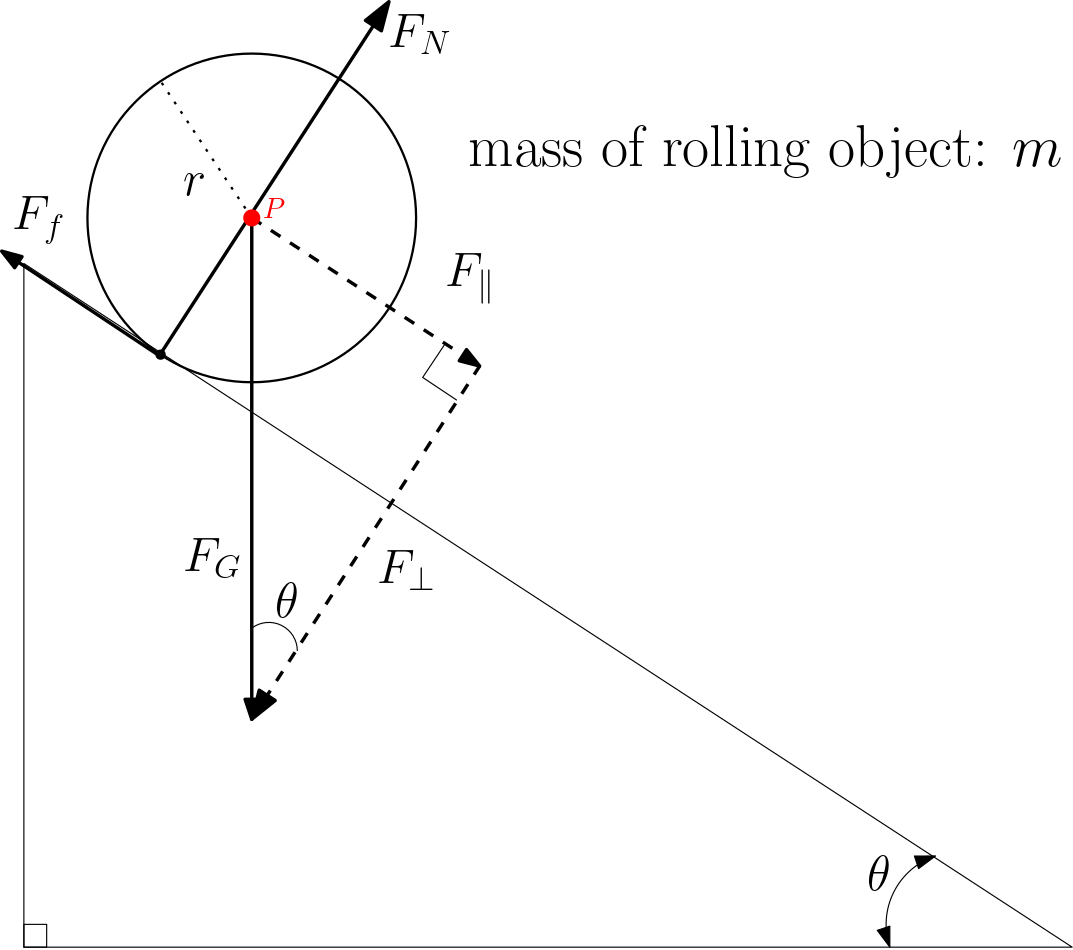
\includegraphics[width=0.5\textwidth]{ramp_incline_labelled}
    \caption{Diagram of rolling object on inclined ramp labelled with forces}
    \label{fig:ramp_labelled}
\end{figure}

Referring to Figure \ref*{fig:ramp_labelled}, the translational $F_{net}$ is given by
$$
    F_{net} = F_{\parallel} - F_f
$$
as every force in the system other than frictional force ($F_f$) and the force component of
gravitational force parallel to the incline of the ramp ($F_{\parallel}$) is being cancelled
out by some other force.

% TODO: bad explanation
The rolling object is also experiencing a torque relative to the point $P$ in Figure \ref*{fig:ramp_labelled}.
This torque is only arising from frictional force, as while $F_N$ passes through
point $P$ and $F_G$ is originating from point $P$, $F_f$ is the only force that is
creating a force that originates from some point other than $P$ and is perpendicular
to the line of the force's own origin to $P$.

Using this information, the formula for the translational acceleration of the two rolling objects
(a hollow cylinder and a solid sphere) can be derived.

\subsection{Derivation of the formula for translational acceleration of the hollow cylinder}

The moment of inertia for a hollow cylinder is $I = mr^2$. The derivation for the
translational acceleration of this cylinder is shown below.

\begin{align*}
     & \Gamma = I\alpha, ~ \Gamma = F_f r, ~ \alpha = \frac{a}{r}
    \\
     & F_f r = mr^2\left(\frac{a}{r}\right)
    \\
     & F_f = ma
    \\
    \\
     & \sin(\theta) = \frac{F_{\parallel}}{F_G}, ~ F_G = mg
    \\
     & F_{\parallel} = mg\sin(\theta)
    \\
    \\
     & F_{net} = ma
    \\
     & F_{\parallel} - F_f = ma
    \\
     & mg\sin(\theta) - ma = ma
    \\
     & a = \frac{1}{2}g\sin{\theta}
\end{align*}

\subsection{Derivation of the formula for translational acceleration of the solid sphere}

The moment of inertia for a hollow cylinder is $I = \frac{2}{5}mr^2$. The derivation for the
translational acceleration of this cylinder is shown below.

\begin{align*}
     & \Gamma = I\alpha, ~ \Gamma = F_f r, ~ \alpha = \frac{a}{r}
    \\
     & F_f r = \frac{2}{5}mr^2\left(\frac{a}{r}\right)
    \\
     & F_f = \frac{2}{5}ma
    \\
    \\
     & \sin(\theta) = \frac{F_{\parallel}}{F_G}, ~ F_G = mg
    \\
     & F_{\parallel} = mg\sin(\theta)
    \\
    \\
     & F_{net} = ma
    \\
     & F_{\parallel} - F_f = ma
    \\
     & mg\sin(\theta) - \frac{2}{5}ma = ma
    \\
     & a = \frac{5}{7}g\sin{\theta}
\end{align*}

\subsection{How the predicted time to reach the end of the ramp is calculated}

Given that we will be able to calculated the angle of inclination of the ramp using
the length and height of the ramp, we will be able to find what the translational
acceleration of the rolling object will be. Additionally, we know the incline
length of the ramp and that the initial translational velocity of the rolling object
will be zero. Since we know the values of $a, u, s$, then we can calculate the
predicted time to reach the end of the ramp.

\begin{align*}
     & s = ut + \frac{1}{2}at^2
    \\
     & \text{Because } u = 0
    \\
     & s = \frac{1}{2}at^2
    \\
     & at^2 = 2s
    \\
     & t^2 = \frac{2s}{a}
    \\
     & t = \sqrt{\frac{2s}{a}}
\end{align*}

\section{Raw data}

\subsection{Qualitative observations}

\begin{figure}[H]
    \centering
    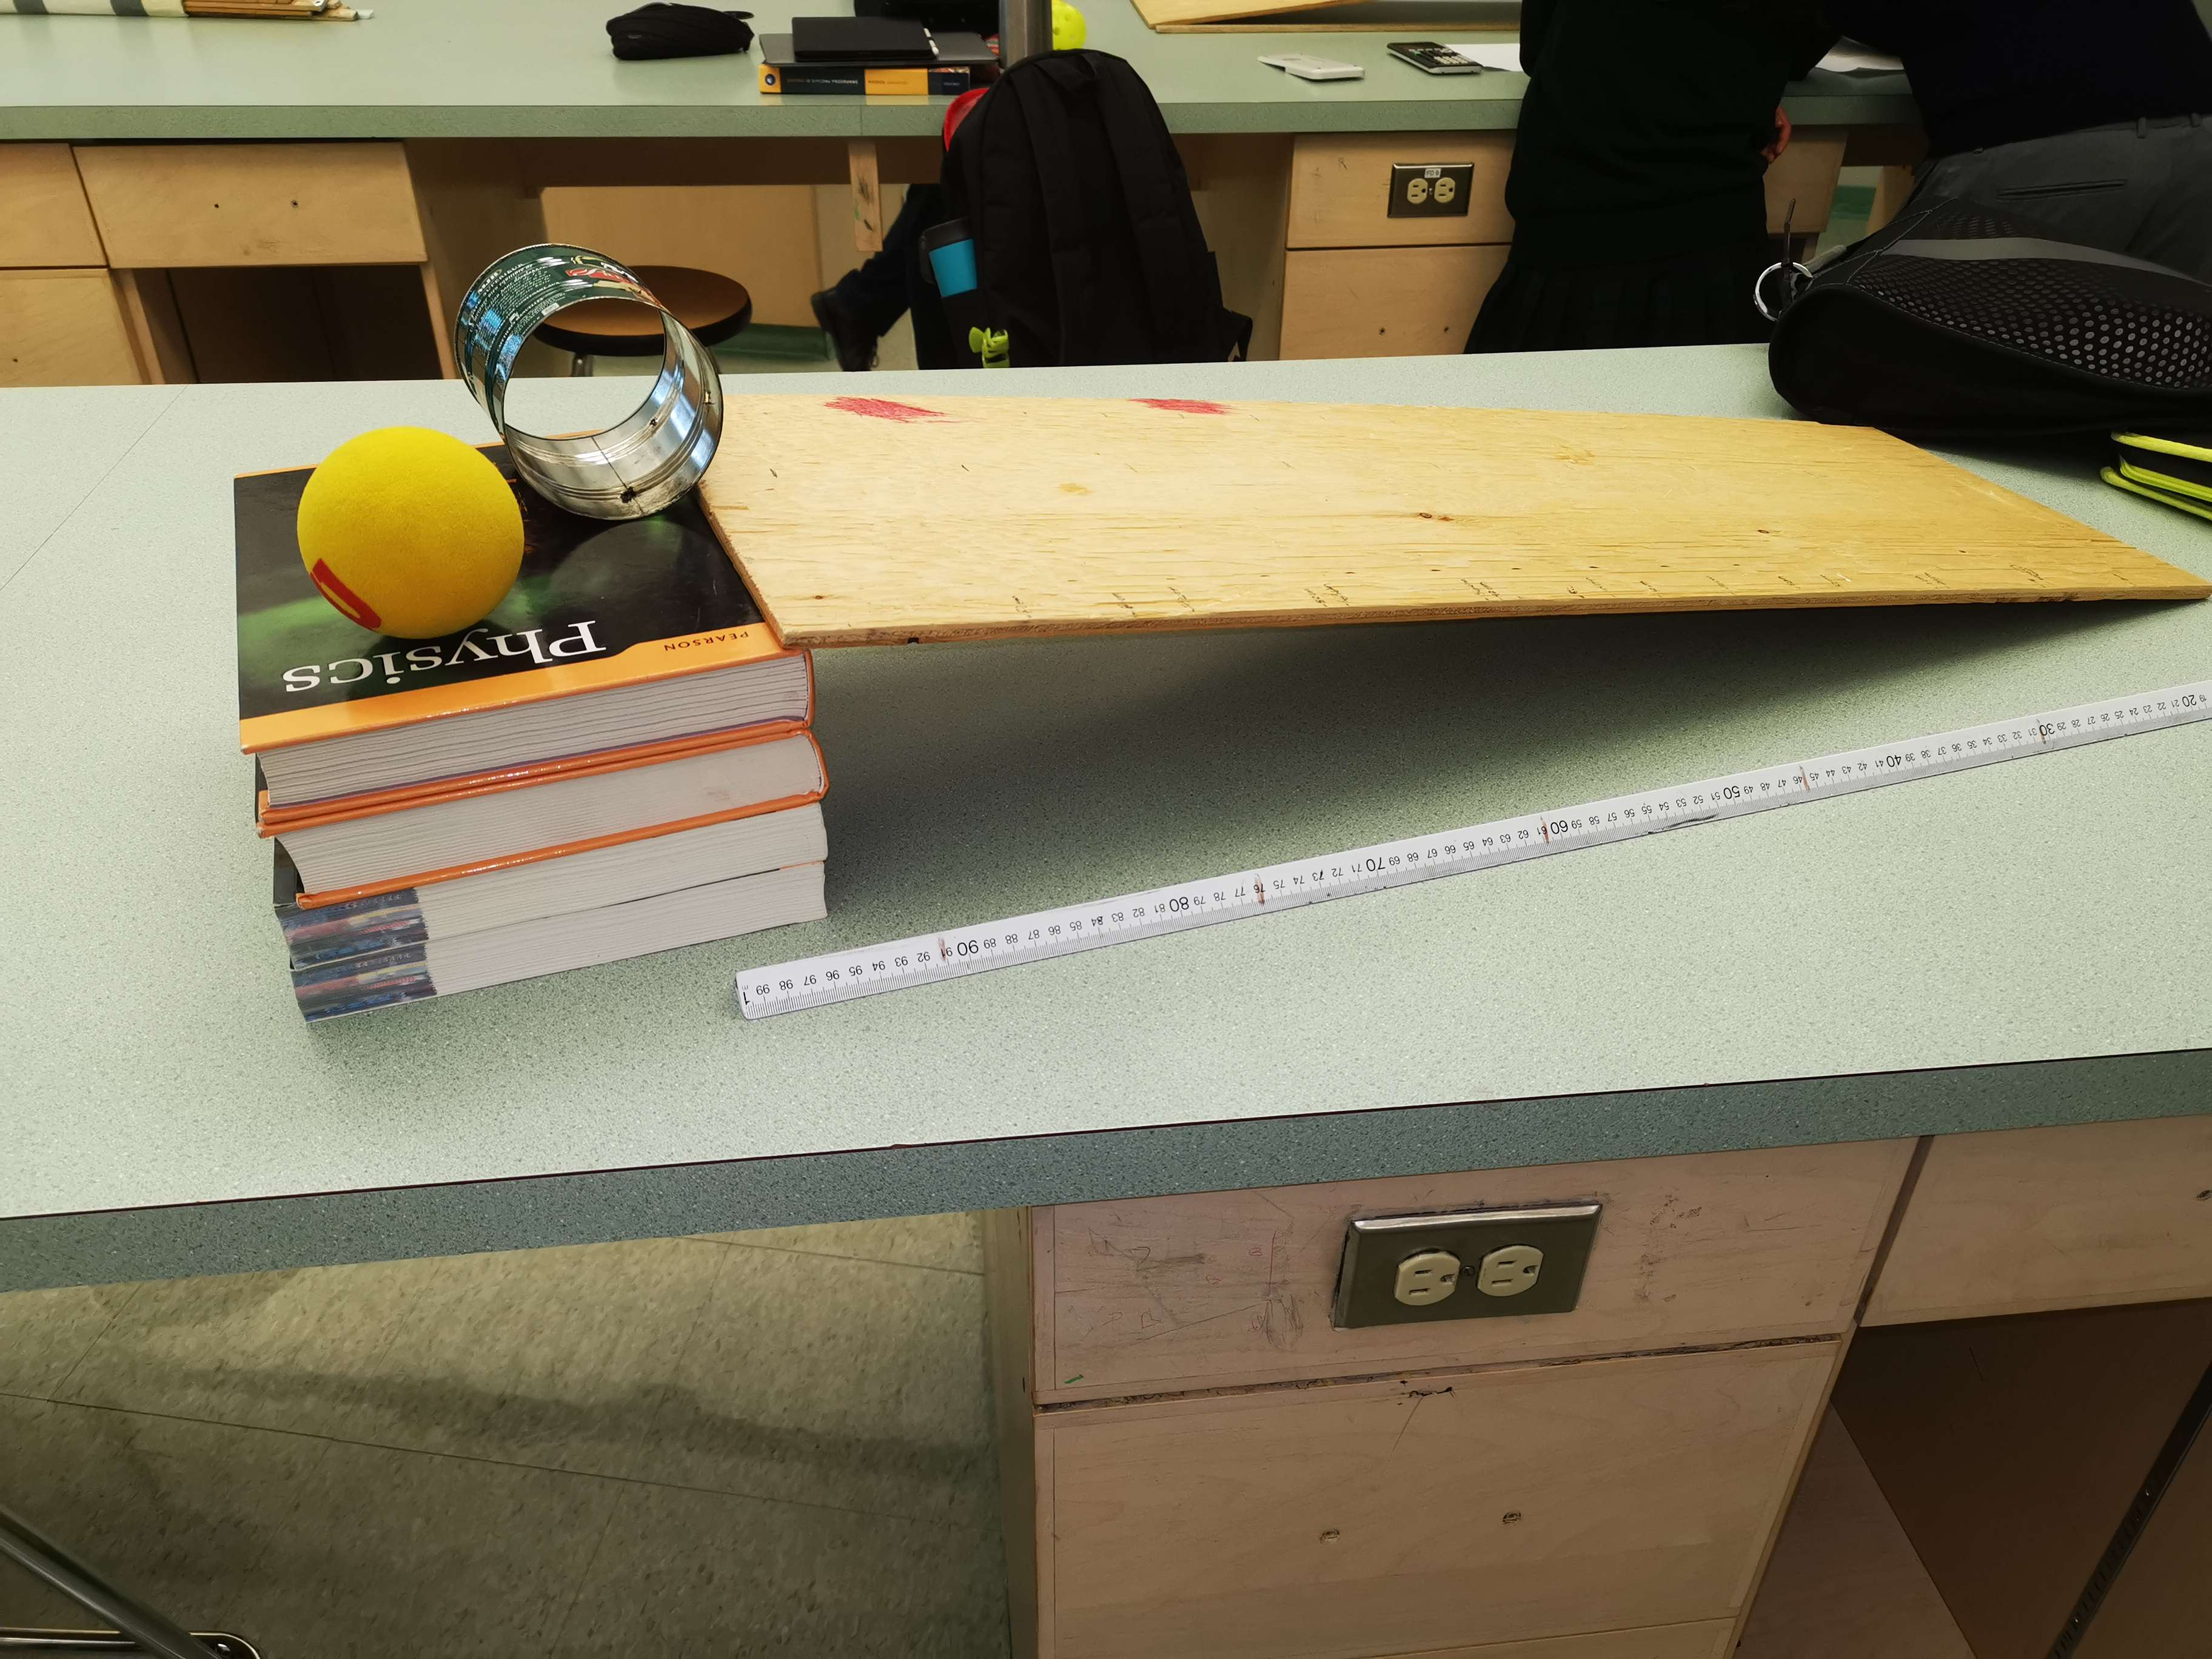
\includegraphics[width=0.5\textwidth]{apparatus}
    \caption{Photo of the sphere, cylinder and ramp}
    \label{fig:apparatus}
\end{figure}

\subsubsection{Hollow cylinder}

Upon close inspection, the hollow cylinder does not appear to be completely circular
and is rather in a slight elliptical shape. This is assumed to be as a result of
the cylinder's malleable material.

Additionally, the cylinder has grooves and holes along the exterior of it. This may
or may not affect the frictional force of the cylinder moving down the ramp.

\subsubsection{Solid sphere}

The solid sphere, being made of foam, is soft and squishy. This may affect the
normal force of the sphere, as rather than only having on point of contact for the
normal force to originate from, the sphere will have a considerable area of contact,
in which various parts of the area of contact will have different magnitudes of
normal force.

When conducting the trials, the sphere was found to sometimes roll diagonally down the
ramp. This may be as a result of the sphere being soft and squishy, causing a larger
area of contact and potentially a normal force directed to one side or another.

The material of foam may also have a slight affect on the moment of inertia of the
sphere, as the air in the sphere may cause a slightly different distribution of mass
in the sphere.

\subsection{Quantitative data}

\begin{table}[H]
    \centering
    \begin{tblr}{
            row{even} = {c},
            row{3} = {c},
            row{5} = {c},
            row{7} = {c},
            row{9} = {c},
            row{11} = {c},
            row{13} = {c},
            row{15} = {c},
            row{17} = {c},
            row{19} = {c},
            row{21} = {c},
            hlines,
            vlines,
        }
        {Time for hollow cylinder \\to roll down ramp /s \\$\Delta t\pm 0.3\unit{s}$} & {Time for solid sphere\\to roll down ramp /s\\$\Delta t\pm 0.2\unit{s}$} \\
        1.4 & 1.2                 \\
        1.4 & 1.5                 \\
        1.5 & 1.6                 \\
        1.6 & 1.5                 \\
        2.0 & 1.6                 \\
        1.6 & 1.3                 \\
        1.7 & 1.4                 \\
        1.6 & 1.3                 \\
        1.7 & 1.3                 \\
        1.7 & 1.5                 \\
        1.7 & 1.5                 \\
        1.6 & 1.6                 \\
        1.6 & 1.5                 \\
        1.7 & 1.4                 \\
        1.8 & 1.5                 \\
        1.6 & 1.5                 \\
        2.0 & 1.4                 \\
        1.7 & 1.6                 \\
        1.7 & 1.4                 \\
        1.7 & 1.5
    \end{tblr}
    \caption{Raw data of time to roll down ramp for both hollow cylinder and solid sphere}
    \label{tab:raw_data}
\end{table}

Phyphox has determined that the angle of inclination when the phone is laid down on
the table is 0.80\degree, and the angle of inclination when put on the ramp
is 10.10\degree.

\section{Processed data}

Note that the values used in the following calculations are unrounded and therefore are not entirely
reflected by Table \ref*{tab:raw_data}.

\subsection{Averaged values}

The averaged values of the time it takes for either the hollow cylinder or
the solid sphere to roll completely down the ramp is calculated using the following
formula:

\begin{align*}
                  & \overline{t} = \frac{\sum t}{n}
    \\
    \text{where } & \overline{t} = \text{ averaged value of all the trials } /\unit{s}
    \\
                  & t = \text{ a single time value of one of the trials } /\unit{s}
    \\
                  & n = \text{ number of trials }
\end{align*}

\subsubsection{Averaged values from raw data for hollow cylinder}

\begin{align*}
     & \overline{t} = \frac{\sum t}{n}
    \\
     & \overline{t} = \frac{33.12 \unit{s}}{20}
    \\
     & = 1.66 \unit{s}
\end{align*}

\subsubsection{Averaged values from raw data for solid sphere}

\begin{align*}
     & \overline{t} = \frac{\sum t}{n}
    \\
     & \overline{t} = \frac{29.19\unit{s}}{20}
    \\
     & = 1.47\unit{s}
\end{align*}

\subsection{Calculation of uncertainty from human error}

The uncertainty for both the timing of the hollow cylinder and
the solid sphere is calculated using the following formula.

$$
    err = \frac{MAX - MIN}{2}
$$

\subsubsection{Uncertainty for hollow cylinder}

The hollow cylinder had a maximum time of 1.99 \unit{s} and a minimum
time of 1.36 \unit{s}. The calculation for the human error uncertainty of the hollow cylinder is
shown below.

\begin{align*}
     & err = \frac{MAX - MIN}{2}
    \\
     & err = \frac{1.99 \unit{s} - 1.36 \unit{s}}{2}
    \\
     & err = 0.315 \unit{s}
    \\
     & err = 0.3 \unit{s}
\end{align*}

\subsubsection{Uncertainty for solid sphere}

The solid sphere had a maximum time of 1.64 \unit{s} and a minimum time of 1.24 \unit{s}.
The calculation for the human error uncertainty of the solid sphere is shown below.

\begin{align*}
     & err = \frac{MAX - MIN}{2}
    \\
     & err = \frac{1.64\unit{s} - 1.24\unit{s}}{2}
    \\
     & err = 0.2\unit{s}
\end{align*}

\subsection{Formal experimental results}

Using the averaged values and calculated uncertainty for both the
hollow cylinder and the solid sphere, the formal experimental results
can be presented.

$$
    \overline{t}_{hollow cylinder} = 1.7 \unit{s} \pm 0.3 \unit{s}
$$

$$
    \overline{t}_{solid sphere} = 1.5 \unit{s} \pm 0.2 \unit{s}
$$


\section{Determining predicted times}

\subsection{Angle of inclination of the ramp}

Given that we know what the height and hypotenuse of the ramp is, we can calculate
the angle of inclination using trigonometry. Note that eventually in our calculation of the predicted times,
we can simply substitute $\sin\theta$ for $\frac{height}{hypotenuse}$.
However, we will nevertheless be calculating the angle of inclination to ensure
that the calculated value is reasonable by comparing it to the angle of inclination
measured by phyphox.

Because there is measurement uncertainty in the height and hypotenuse of the ramp,
we will approach calculating the angle of inclination by determining the maximum
and minimum value of the angle of inclination.

The height of the ramp is $14.70\unit{cm} \pm 0.05\unit{cm}$, and the
hypotenuse of the ramp is $90.90\unit{cm} \pm 0.05\unit{cm}$.

\begin{align*}
     & \theta_{max} = \sin^{-1}\left(\frac{height}{hypotenuse}\right)
    \\
     & = \sin^{-1}\left(\frac{14.75\unit{cm}}{90.85\unit{cm}}\right)
    \\
     & = 9.3436\degree
    \\
     & = 9.34\degree
    \\
    \\
     & \theta_{min} = \sin^{-1}\left(\frac{height}{hypotenuse}\right)
    \\
     & = \sin^{-1}\left(\frac{14.65\unit{cm}}{90.95\unit{cm}}\right)
    \\
     & = 9.2694\degree
    \\
     & = 9.27\degree
\end{align*}

The averaged value and absolute error of the maximum and minimum values
will then be calculated.

\begin{align*}
     & \theta = \frac{\theta_{max} + \theta_{min}}{2}
    \\
     & = \frac{9.3436\degree + 9.2694\degree}{2}
    \\
     & = 9.3065\degree
    \\
     & = 9.31\degree
    \\
    \\
     & err = \frac{\theta_{max} - \theta_{min}}{2}
    \\
     & = \frac{9.3436\degree - 9.2694\degree}{2}
    \\
     & = 0.0371\degree
    \\
     & = 0.04\degree
\end{align*}

The angle of inclination can then be presented as:
$$
    \theta = 9.31\degree \pm 0.04\degree
$$

Phyphox measured that the angle of inclination of the table was 0.80\degree
and the angle of inclination of the ramp was 10.10\degree. By subtracting
these values, we determine that the angle of inclination between the table
and the ramp is 9.30\degree, indicating that the angle of inclination
calculated through trigonometry is reasonable as the value of 9.30\degree
fits within the range of $9.31\degree \pm 0.04\degree$.

\subsection{Calculating predicted time for hollow cylinder}

Recalling the following formulas for the hollow cylinder:
\begin{equation}
    a = \frac{1}{2}g\sin\theta
\end{equation}
\begin{equation}
    t = \sqrt{\frac{2s}{a}}
\end{equation}

By substituting Equation 1 for $a$ in Equation 2, we derive the formula:

$$
    t = \sqrt{\frac{4s}{g\sin\theta}}
$$

\section{Comparing experimental times to predicted times}


\end{document}